\documentclass{beamer}

\usepackage{amssymb}
\usepackage{amsmath}
\usepackage{amsthm}
\usepackage{amsfonts}

\usepackage{multicol}

\usepackage{graphicx}
\graphicspath{ {./src} }

\usepackage{tikz}

\usepackage{pgfplots}
\pgfplotsset{compat = newest}

\usepackage{verbatim}
\usetikzlibrary{arrows,shapes}

% for cross reference
% \usepackage{hyperref}

% for fixed length of cell of tables
% \usepackage{tabularx}
% \usepackage{longtable}

\AtBeginSection[]
{
  \begin{frame}
    \frametitle{Table of Contents}
    \tableofcontents[currentsection]
  \end{frame}
}

\title{Communicate Without Errors}
\author{Zifan Hua}

\begin{document}

      \frame{\titlepage}

      \begin{frame}
            \frametitle[TOC]{Table Of Contents}
            \tableofcontents
      \end{frame}

      \section{Introduction}

      \begin{frame}
            \frametitle{Introduction}
            \begin{itemize}
                  \item Channel Capacity
                  \item Zero Error Rate
                  \item Shannon Capacity
                  \item $C_{n}$
            \end{itemize}
      \end{frame}

      \section{Some Definitions}

            \subsection{Channel}

                  \begin{frame}
                        \frametitle{Channel}
                        \begin{definition}[channel]
                              A channel has a sender and a receiver.
                              \pause

                              The sender sends a finite sequence of characters to the receiver which is called message.
                              \begin{figure}[h!]
                                    \tikzstyle{vertex}=[fill=black!25,minimum size=20pt,inner sep=0pt]
                                    \tikzstyle{message}=[inner sep=0pt]
                                    \tikzstyle{edge} = [draw,thick,-]
                                    \tikzstyle{weight} = [font=\small]
                                    \begin{tikzpicture}[scale=1, auto,swap]
                                          % Draw a 7,11 network
                                          % First we draw the vertices
                                          \foreach \pos/\name in {{(0,0)/sender}, {(3,0)/receiver}}
                                                \node[vertex] (\name) at \pos {$\name$};
                                          \foreach \pos/\name in {{(0,1)/abcde}, {(3,1)/acbde}}
                                                \node[message] (\name) at \pos {$\name$};
                                          % Connect vertices with edges and draw weights
                                          \foreach \source/ \dest in {sender/receiver}
                                          \path[edge] (\source) -- node[weight]{} (\dest);
                                    \end{tikzpicture}
                              \end{figure}
                              \pause
                              
                              The receiver receives the sequence of characters and decode it.
                              \pause

                              However, in the procedure of send and receive, the channel may introduce some errors. For instance, here, $b$ is decoded into $c$. 

                              Worth to note that this may not be "abelian". Which means $b$ have chance to be decoded into $c$, but $c$ may not have the chance to be decoded into $b$.
                        \end{definition}
                  \end{frame}

                  \begin{frame}
                        \frametitle{Channel}
                        \begin{definition}[confusable]
                              Given two characters $a$, $b$. If $a$ and $b$ have chance to be decoded into a same character say $c$, we say $a$ and $b$ are confusable.

                              For a two messages of length $n$, we say that they are confusable if the two messages can be decoded into the same message.
                        \end{definition}
                        \pause
                        \begin{definition}[rate of channel]
                              Given a channel that could send $m$ distinct messages with length $n$.
                              And could be able to send only one character per unit time.
                              The rate of channel is $\sqrt[n]{m}$.

                              Here, we do not care about how much characters we have or how many characters we used. We only care about the number of all messages we can send.
                              
                        \end{definition}
                  \end{frame}

                  \begin{frame}
                        \frametitle{Channel}
                        \begin{definition}[zero error rate]
                              Given a channel which could transfer messages of length $n$.

                              We want to find the maximum set of messages $M$ that no two of them is confusable.

                              \begin{equation}
                                    \text{zero error rate} = \max_{M} \sqrt[n]{|M|}
                              \end{equation}
                        \end{definition}
                  \end{frame}

                  \begin{frame}
                        \frametitle{Channel}
                        If given a set of characters $S$, and some of the characters could be confusable.

                        We want to find
                        \begin{equation}
                              \sup_{n} \left\{
                                    \text{zero error rate of channel with length $n$ and $S$ as characters}
                              \right\}
                        \end{equation}
                  \end{frame}

            \subsection{Graph Representation of Characters}

                  \begin{frame}
                        \frametitle{Graph Representation Of Characters}
                        \begin{definition}[graph] \label{def:graph}
                              A graph $ G $ is a set of vertices with a set of edges connecting pairs of vertices.

                              \begin{figure}[h!]
                                    \tikzstyle{vertex}=[circle,fill=black!25,minimum size=20pt,inner sep=0pt]
                                    \tikzstyle{edge} = [draw,thick,-]
                                    \tikzstyle{weight} = [font=\small]
                                    \begin{tikzpicture}[scale=1, auto,swap]
                                          % Draw a 7,11 network
                                          % First we draw the vertices
                                          \foreach \pos/\name in {{(0,2)/a}, {(2,1)/b}, {(4,1)/c},
                                                {(0,0)/d}, {(3,0)/e}, {(2,-1)/f}, {(4,-1)/g}}
                                                \node[vertex] (\name) at \pos {$\name$};
                                          % Connect vertices with edges and draw weights
                                          \foreach \source/ \dest in {b/a, c/b,d/a,d/b,
                                                e/b, e/c,e/d,
                                                f/d,f/e,
                                                g/e,g/f}
                                          \path[edge] (\source) -- node[weight]{} (\dest);
                                    \end{tikzpicture}
                                    \label{fig:graphDefinitionExample}
                                    \caption{An example of a graph.}
                              \end{figure}
                        \end{definition}
                  \end{frame}

                  \begin{frame}
                        \frametitle{Graph Representation Of Characters}
                        \begin{definition}\label{def:graphRepresetationOfChannel}
                              Given a channel that sending $\{1,2,\dots,n\}$ as characters. And some characters $i$ and $j$ could be confused with each other.

                              \pause

                              Then the graph representation of the characters is the graph with vertices $\{1,2,\dots,n\}$ and edges $(i,j)$ if and only if $i$ and $j$ could be confused with each other.
                        \end{definition}
                  \end{frame}

            \subsection{Alpha Function}

                  \begin{frame}
                        \frametitle{$\alpha(G)$}
                        \begin{definition}[$\alpha(G)$]\label{def:alpha}
                              The $\alpha(G)$ represent the maximum number of characters that could not be confused with each other in graph $G$.

                              \pause

                              Given a graph $ G $. Given a subgraph $ H $ of $ G $, such that every vertex of $ H $ is not connected in $ G $. Then $ \alpha(G) $ is the maximum number of vertices of $ H $.
                              \tikzstyle{vertex}=[circle,fill=black!25,minimum size=20pt,inner sep=0pt]
                              \tikzstyle{selected vertex}=[circle,fill=red!25,minimum size=20pt,inner sep=0pt]
                              \tikzstyle{edge} = [draw,thick,-]
                              \tikzstyle{weight} = [font=\small]
                              \begin{figure}[h!]
                                    \begin{tikzpicture}[scale=1, auto,swap]
                                          % Draw a 7,11 network
                                          % First we draw the vertices
                                          \foreach \pos/\name in {{(0,2)/a}, {(2,1)/b}, {(4,1)/c},
                                                {(0,0)/d}, {(3,0)/e}, {(2,-1)/f}, {(4,-1)/g}}
                                                \node[vertex] (\name) at \pos {$\name$};
                                          \foreach \pos/\name in {{(0,2)/a}, {(4,1)/c},
                                                {(2,-1)/f}}
                                                \node[selected vertex] (\name) at \pos {$\name$};
                                          % Connect vertices with edges and draw weights
                                          \foreach \source/ \dest in {b/a, c/b,d/a,d/b,
                                                e/b, e/c,e/d,
                                                f/d,f/e,
                                                g/e,g/f}
                                          \path[edge] (\source) -- node[weight]{} (\dest);
                                    \end{tikzpicture}
                                    \label{fig:alphaGExample}
                                    \caption{Example of $ \alpha(G) $. Here $ \alpha(G) = 3 $.}
                              \end{figure}
                        \end{definition}
                  \end{frame}

            \subsection{Product Graph}

                  \begin{frame}
                        \frametitle{Product Graph}
                        \begin{definition}[graph product]\label{def:graphProduct}
                              The product of two graphs can be considered as send a pair of characters $(x,y)$ as one character or one message.

                              \pause

                              Given two graph $ G $ and $ H $. The graph product $ G \times H $ is the graph with vertices $ V(G \times H) = V(G) \times V(H) $ in which $ (x,y) $ is adjacent to $ (x',y') $ in $ G \times H $ if and only if $ x $ is adjacent to $ x' $ in $ G $ and $ y $ is adjacent to $ y' $ in $ H $.
                  
                              \pause

                              A graph $ G $ product itself for $ n $ times will always be denoted by $ G^n $.
                        \end{definition}
                  \end{frame}

                  \begin{frame}
                        \frametitle{Properties of $\alpha(g)$}
                        \begin{lemma}
                              $\alpha(G)\alpha(H) \leq \alpha(G \times H)$
                        \end{lemma}

                        \pause

                        \begin{proof}
                              Given graph $ G $ and $ H $. Let $ G' $ and $ H' $ be subgraph of $ G $ and $ H $ such that no vertex of $ G' $ or $ H' $ is adjacent in $ G $ or $ H $, respectively. Then $ G' \times H' $ is a subgraph of $ G \times H $ such that no vertex of $ G' \times H' $ is adjacent in $ G \times H $.
                        \end{proof}
                  \end{frame}

            \subsection{Shannon Capacity}

                  \begin{frame}
                        \frametitle{Shannon Capacity}
                        \begin{definition}[Shannon Capacity]\label{def:shannonCapacity}
                              The Shannon capacity of a channel is defined on sending a series if characters.

                              \pause

                              Given a graph $ G $, the Shannon capacity $ \Theta(G) $ is defined by
                              \begin{equation}
                                    \Theta(G) = \sup_{n} \sqrt[n]{\alpha(G^n)} 
                              \end{equation}

                              \pause

                              We will see that this sequence has an upper bound later. 
                        \end{definition}
                  \end{frame}

            \subsection{Orthonormal Representation}

                  \begin{frame}
                        \frametitle{Orthonormal Representation}
                        \begin{definition}[Orthonormal Representation]\label{def:orthonormalRepresentation}
                              Given a graph $ G $ with vertices $ 1,2,\dots,n $, the orthonormal representation of $ G $ is a set of unit vectors $ \{v_1, v_2, \dots, v_n\} $ such that $ v_i $ and $ v_j $ are orthogonal if $ i $ and $ j $ are not adjacent in $ G $.
                        \end{definition}

                        \pause

                        Any orthonormal basis of $ \mathbb{R}^n $ can be used as an orthonormal representation of $ G $. So, for any graph $ G $, there exist some orthonormal representations.
                  \end{frame}

                  \begin{frame}
                        \frametitle{Tensor Product}
                        \begin{definition}[tensor product]\label{def:tensorProduct}
                              Given two vectors $ v = \left(v_{1},\dots,v_{n}\right) $ and $ w = \left(w_{1},\dots,w_{n}\right) $, the tensor product $ v \circ w $ is defined by
                              \begin{equation}
                                    v \circ w = \left(
                                          v_{1}w_{1},\dots,v_{1}w_{n},
                                          v_{2}w_{1},\dots,v_{2}w_{n},
                                          \dots,
                                          v_{n}w_{1},\dots,v_{n}w_{n}
                                          \right)
                              \end{equation}
                        \end{definition}

                        \pause

                        \begin{lemma}
                              The inner product of tensor products can be computed by,
                              \begin{equation}
                                    \langle v \circ w, v' \circ w' \rangle = \langle v, v' \rangle \langle w, w' \rangle
                              \end{equation}
                        \end{lemma}

                  \end{frame}

                  \begin{frame}
                        \frametitle{Product of Orthonormal Representation}
                        \begin{lemma}
                              Given a graph $ G $ with vertices $ 1,2,\dots,n $, and a graph $ H $ with vertices $ 1,2,\dots,m $. Then vectors $\{ v_{i}\circ w_{j} \}$ is an orthonormal representation of $ G \times H $.
                        \end{lemma}
                  \end{frame}

            \subsection{Theta Function}

                  \begin{frame}
                        \frametitle{Theta Function}
                        Given a graph $ G $, the $ \theta(G) $ is defined by
                        \begin{equation}
                              \theta(G) = \inf_{\{v_1, v_2, \dots, v_n\},c} \max_{i} \frac{1}{\left<c,v_{i}\right>^2}
                        \end{equation}
                        where $ \{v_1, v_2, \dots, v_n\} $ is an orthonormal representation of $ G $, and c is any unit vector does not orthogonal to $ v_i $.

                        \pause

                        \begin{lemma}
                              There always exist such an $c$ and orthonormal representation $ \{v_1, v_2, \dots, v_n\} $ such that
                              \begin{equation}
                                    \theta(G) = \max_{i} \frac{1}{\left<c,v_{i}\right>^2}
                              \end{equation}
                        \end{lemma}

                        This could be proved by proving the set of all possible cases of $ \{v_1, v_2, \dots, v_n,c \} $ is compact. And the function $ \max \frac{1}{\left<c,v_{i}\right>^2} $ is continuous.
                  \end{frame}

                  \begin{frame}
                        \frametitle{Theta Function}
                        \begin{lemma}
                              Given graph $ G $ and $ H $, then
                              \begin{equation}
                                    \theta(G \times H) \leq \theta(G) \theta(H)
                              \end{equation}
                        \end{lemma}

                        \pause

                        \begin{proof}
                              Let $ \{v_1, v_2, \dots, v_n\} $ and $ \{w_1, w_2, \dots, w_m\} $ be orthonormal representation of $ G $ and $ H $ and $ c_{v} $ and $ c_{w} $ such that
                              \begin{equation}
                                    \max \left\{ \frac{1}{\left<c_{v},v_{i}\right>^2} : i=1,2,\dots,n \right\} = \theta(G)
                              \end{equation} 
                              and 
                              \begin{equation}
                                    \max \left\{ \frac{1}{\left<c_{w},w_{i}\right>^2} : i=1,2,\dots,m \right\} = \theta(H)
                              \end{equation}
                        \end{proof}
                  \end{frame}

                  \begin{frame}
                        \begin{proof}
                              Then
                              \begin{eqnarray}
                                    \theta(G \times H) &\leq& 
                                    \max \left\{ \frac{1}{\left<c_{v} \circ c_{w},v_{i} \circ w_{j}\right>^2} \right\} \\
                                    &=& \max \left\{ \frac{1}{\left<c_{v},v_{i}\right>^2 \left<c_{w},w_{j}\right>^2} \right\} \\
                                    &=& \max \left\{ \frac{1}{\left<c_{v},v_{i}\right>^2} \right\} \max \left\{ \frac{1}{\left<c_{w},w_{j}\right>^2} \right\} \\
                                    &=& \theta(G) \theta(H) \\
                              \end{eqnarray}
                        \end{proof}
                  \end{frame}

      \section{Some Theorems of Linear Algebra}

            \begin{frame}
                  \begin{theorem}[Spectral Theorem]
                        \begin{itemize}
                              \item Let $T$ be a symmetric operator on a Euclidean space $V$.
                              \begin{itemize}
                                    \item There exist an orthonormal basis of $V$ consisting of eigenvectors of $T$.
                                    \item The eigenvalues of $T$ are real numbers.
                              \end{itemize}
                              \item Let $A$ be a real symmetric matrix.
                              \begin{itemize}
                                    \item There exist an orthogonal matrix $P$ such that $P^TAP$ is a real diagonal matrix.
                                    \item The eigenvalues of $A$ are real numbers.
                              \end{itemize}
                        \end{itemize}
                  \end{theorem}
            \end{frame}

      \section{The Real Question}

            \subsection{Lemma 1}

                  \begin{frame}
                        \begin{lemma}
                              \begin{equation}
                                    \theta(G) \geq \alpha(G)
                              \end{equation}
                        \end{lemma}

                        \pause

                        \begin{proof}
                              Let $ \{1,2,\dots,k\} $ be the set of vertices of $ G $ such that every point is not adjacency in $ G $. And $ k = \alpha(G) $
                  
                              Let $ \{v_1, v_2, \dots, v_n\} $ be an orthonormal representation of $ G $ and $ c $ such that
                              \begin{equation}
                                    \max \left\{ \frac{1}{\left<c,v_{i}\right>^2} \right\} = \theta(G)
                              \end{equation}
                                    
                              Then
                              \begin{eqnarray}
                                    1 &=& c^{2}
                                    \geq \sum_{i=1}^{k} \left<c,v_{i}\right>^{2}
                                    \geq \frac{k}{\theta(G)}
                              \end{eqnarray}
                        \end{proof}
                  \end{frame}

            \subsection{Theorem 1}
                  
                  \begin{frame}
                        \begin{theorem}
                              Given a graph $ G $, then
                              \begin{equation}
                                    \theta(G) \geq \Theta(G)
                              \end{equation}
                        \end{theorem}

                        \pause

                        \begin{proof}
                              \begin{eqnarray}
                                    \Theta(G) &=& \lim_{n} \sqrt[n]{\alpha(G^{n})} \\
                                    &\leq& \lim_{n} \sqrt[n]{\theta(G^{n})} \\
                                    &\leq& \lim_{n} \sqrt[n]{\theta(G)^{n}} \\
                                    &=& \theta(G)
                              \end{eqnarray}
                        \end{proof}
                  \end{frame}

                  \begin{frame}
                        The final result we want to prove today,
                        \begin{equation}
                              \Theta(C_{5}) \le \theta(C_{5}) \le \sqrt{5}
                        \end{equation}
                  \end{frame}

            \subsection{Theorem 2}

                  \begin{frame}
                        \begin{theorem}
                              \begin{equation}
                                    \theta(C_{n}) \leq \sqrt{5}
                              \end{equation}
                        \end{theorem}
                  \end{frame}

                  \begin{frame}
                        \begin{proof}
                              Consider an umbrella that has a handle and $5$ ribs that all have unit length. And also its handle is a unit vector.
                  
                              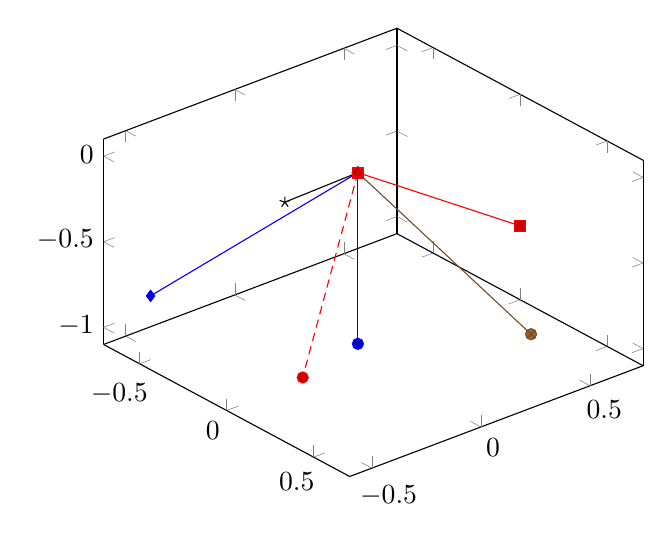
\begin{tikzpicture}
                   
                                    \begin{axis}[view = {50}{40}]
                                     
                                    \addplot3 coordinates 
                                    {
                                        (0,0,0)
                                        (0,0,-1)
                                    };
                  
                                    \addplot3 coordinates 
                                    {
                                        (0,0,0)
                                        (0,0.74349606,-0.66874031)
                                    };
                                     
                                    \addplot3 coordinates 
                                    {
                                        (0,0,0)
                                        (0.70710677,0.22975292,-0.66874031)
                                    };
                  
                                    \addplot3 coordinates 
                                    {
                                        (0,0,0)
                                        (-0.70710677,0.22975292,-0.66874031)
                                    };
                  
                  
                                    \addplot3 coordinates 
                                    {
                                        (0,0,0)
                                        (-0.43701602,-0.60150095,-0.66874031)
                                    };
                                    
                                    \addplot3 coordinates 
                                    {
                                        (0,0,0)
                                        (0.43701602,-0.60150095,-0.66874031)
                                    };
                  
                                    \end{axis}
                                     
                              \end{tikzpicture}

                        \end{proof}
                  \end{frame}

                  \begin{frame}
                        \begin{proof}
                              Here, angles between two consecutive ribs are same. 
                              
                              Let $v$ be a rib. And let $w$ be one of the rib that have the largest angle with $v$. Then, we let the angle between $v$ and $w$ be $ \pi/2 $.
                  
                              Then, the $5$ ribs of such an umbrella form an orthonormal representation of $C_{5}$.
                  
                              Let $d$ be the vector represent the handle, and $v_{1},v_{2},\dots,v_{5}$ be the $5$ ribs. And let $\gamma$ be the angle between the handle and any rib.
                  
                              So, by some calculation, we get
                              \begin{eqnarray}
                                    \theta(C_{5}) &\le& \max \frac{1}{<d,v_{i}>^{2}} \\
                                    &=& \left(
                                          \frac{1}{\cos(\gamma)}
                                    \right)^{2} \\
                                    &=& \sqrt{5}
                              \end{eqnarray}
                        \end{proof}
                  \end{frame}
                  
            \subsection{Theorem 3}
                  
                  \begin{frame}
                        \begin{theorem}
                              Let $ G $ be a graph with $ n $ vertices. Let $A=(a_{i,j})$ be a symmetric matrix such that
                              \begin{equation}
                                    a_{i,j} = \left\{
                                          \begin{array}{ll}
                                                1 & \text{if $ i = j $ or $ i $ and $ j $ are not adjacent in $ G $} \\
                                                \text{arbitrary} & \text{otherwise}
                                          \end{array}
                                    \right.
                              \end{equation} 

                              Then
                              \begin{equation}
                                    \theta(G) \le \max\{\text{eigenvalues of $A$}\}
                              \end{equation}
                        \end{theorem}

                        This theorem gives us some way to estimate or even compute the value of $\theta(G)$ in some special cases.
                  \end{frame}

                  \begin{frame}
                        \begin{proof}
                              Let $A$ be a matrix satisfying the requirement. Let $\lambda$ be its largest eigenvalue.
                              Then $\lambda I -A$ is positive semidefinite, and thus exits vectors $\{x_{1},x_{2},\dots,x_{n}\}$ such that
                              \begin{equation}
                                    \lambda\delta_{i,j} - a_{i,j} = \left<x_{i},x_{j}\right>
                              \end{equation}

                              Let $c$ be a unit vector perpendicular to $x_{i}$, and let,\footnote{
                                    Why such $c$ and $\{x_{1},x_{2},\dots,x_{n}\}$ exist, will need some linear algebra. If we have time, we could come back to here.
                              }
                              \begin{equation}
                                    u_{i} = \frac{c+x_{i}}{\sqrt{\lambda}}
                              \end{equation}

                              We will prove that $u_{i}$ is an orthonormal representation of $G$. And also we have 
                              \begin{equation}
                                    \frac{1}{<c,u_{i}>^{2}} = \lambda
                              \end{equation}

                              So, \begin{math}
                                    \theta(G) \le \lambda = \max\{\text{eigenvalues of $A$}\}
                              \end{math}
                        \end{proof}
                  \end{frame}

                  \begin{frame}
                        \begin{proof}
                              Then
                              \begin{eqnarray}
                                    <u_{i},u_{i}> &=& \frac{1}{\lambda} \left<c+x_{i},c+x_{i}\right> \\
                                    &=& \frac{1}{\lambda} (\left<x_{i},x_{i}\right> + 1) \\
                                    &=& \frac{1}{\lambda} (\lambda - 1 + 1) \\
                                    &=& 1
                              \end{eqnarray}

                              Also, for nonadjacent $i$ and $j$,
                              \begin{eqnarray}
                                    <u_{i},u_{j}> &=& \frac{1}{\lambda} \left<c+x_{i},c+x_{j}\right> \\
                                    &=& \frac{1}{\lambda} (\left<x_{i},x_{j}\right>+1) \\
                                    &=& 0
                              \end{eqnarray}
                        \end{proof}
                  \end{frame}

            \subsection{Theorem 4}

                  \begin{frame}
                        \frametitle{Adjacency Matrix}
                        \begin{definition}[Adjacency Matrix]\label{def:adjacencyMatrix}
                              Given a graph $ G $ with vertices $\{1,2,\dots,n\}$, the adjacency matrix $ A $ is defined by
                              \begin{equation}
                                    A_{ij} = \begin{cases}
                                          1 & \text{if $ i $ and $ j $ is adjacent in $ G $} \\
                                          0 & \text{otherwise}
                                    \end{cases}
                              \end{equation}
                        \end{definition}
                        \begin{multicols}{2}
                              \begin{figure}[h!]
                                    \tikzstyle{vertex}=[circle,fill=black!25,minimum size=20pt,inner sep=0pt]
                                    \tikzstyle{edge} = [draw,thick,-]
                                    \tikzstyle{weight} = [font=\small]
                                    \begin{tikzpicture}[scale=1, auto,swap]
                                          % Draw a 7,11 network
                                          % First we draw the vertices
                                          \foreach \pos/\name in {{(0,2)/1}, {(2,2)/2}, {(2,0)/3}, {(0,0)/4}}
                                                \node[vertex] (\name) at \pos {$\name$};
                                          % Connect vertices with edges and draw weights
                                          \foreach \source/ \dest in {1/2, 2/3, 3/4, 4/1}
                                          \path[edge] (\source) -- node[weight]{} (\dest);
                                    \end{tikzpicture}

                                    \begin{equation*}
                                                A = \begin{bmatrix}
                                                      1 & 1 & 0 & 1 \\
                                                      1 & 1 & 1 & 0 \\
                                                      0 & 1 & 1 & 1 \\
                                                      1 & 0 & 1 & 1 \\
                                                \end{bmatrix}
                                    \end{equation*}
                              \end{figure}
                        \end{multicols}
                  \end{frame}

                  \begin{frame}
                        \frametitle{Regular Graph}
                        \begin{definition}[regular graph]
                              A regular graph is a graph where each vertex has the same number of neighbors.
                        \end{definition}
                  \end{frame}
            
                  \begin{frame}
                        \begin{theorem}
                              Let $G$ be a regular graph, and let $\lambda_{1},\lambda_{2},\dots,\lambda_{n}$ be the eigenvalues of its adjacency matrix $A$. Then
                              \begin{equation}
                                    \theta(G) \le n\frac{1-\lambda_{n}}{\lambda_{1}-\lambda_{n}}
                              \end{equation}
                        \end{theorem}

                        This theorem actually gives us a really good estimate of $\theta(G)$ for regular graphs.

                        \pause

                        Also, as $C_{n}$ is a regular graph, and its adjacency graph is a circulant matrix, we could actually compute \begin{math}
                              n\frac{1-\lambda_{n}}{\lambda_{1}-\lambda_{n}}
                        \end{math} for $C_{n}$.

                        And we could get the result we want 
                        \begin{equation}
                              \theta(C_{n}) \le \frac{
                                    n \cos(\pi/n)
                              }{
                                    1+\cos(\pi/n)
                              }
                        \end{equation}
                  \end{frame}

                  \begin{frame}
                        Here we let $J$ be the matrix with all entries equal to $1$.

                        \begin{proof}
                              Consider the matrix $J - x(A-I)$ where $x$ is a real number. Then $J - x(A-I)$ actually met the demand of the proceeding theorem. So, its largest eigenvalue is greater or equal then $\theta(G)$.

                              Let the eigenvalues of $A$ be $\lambda_{1}\ge\lambda_{2}\ge\dots\ge\lambda_{n}$. We could actually proof that eigenvalues of $J - x(A-I)$ are $n-\lambda_{1}x+x,-\lambda_{2}x+x,-\lambda_{3}x+x,\dots,-\lambda_{n}x+x$. 
                              
                              So, the largest eigenvalue of $J - x(A-I)$ is either $n-\lambda_{1}x+x$ or $-\lambda_{n}x+x$.

                              Then, choose $x$ to be
                              \begin{equation}
                                    x = \frac{n}{\lambda_{1}-\lambda_{n}}
                              \end{equation}

                              Then
                              \begin{equation}
                                    \theta(G) \le n\frac{1-\lambda_{n}}{\lambda_{1}-\lambda_{n}}
                              \end{equation}
                        \end{proof}
                  \end{frame}

                  \begin{frame}
                        Here we let $j$ be the vector with all entries equal to $1$.

                        \begin{proof}
                              So, here we proof that eigenvalues of $J - x(A-I)$ are $n-\lambda_{1}x+x,-\lambda_{2}x+x,-\lambda_{3}x+x,\dots,-\lambda_{n}x+x$. 

                              As, $G$ is a regular graph, so suppose every vertex of $G$ has $k$ neighbors, which represent in its adjacency matrix $A$ is that every row or every column of $A$ has exactly $k+1$ ones and others are zeros.

                              So, clearly $j$ is a eigenvector of $A$ with eigenvalue $k+1$. And also $j$ is a eigenvector of $J$ with eigenvalue $n$.

                        \end{proof}
                  \end{frame}

                  \begin{frame}
                        \begin{proof}
                              Next, we will prove that $\lambda_{1} = k+1$

                              Suppose, $w$ is a eigenvector of $A$ with eigenvalue $\lambda > k+1$. Let $w_{i}$ be the entry of $w$ that have the largest absolute value. And $r$ be the $i^{th}$ row of $A$. Then
                              \begin{eqnarray}
                                    \left|\lambda w_{i}\right| &=& \left|\sum_{j=1}^{n}r_{j}w_{j}\right| \\
                                    &=& \left|\sum_{r_{j} \neq 0}w_{j}\right| \\
                                    &\le& \sum_{r_{j} \neq 0}\left|w_{j}\right| \\
                                    &\le& (k+1) \left|w_{i}\right|
                              \end{eqnarray}

                              Contradiction, so $\lambda_{1} = k+1$. So, $n-\lambda_{1}+x$ is an eigenvalue of $J - x(A-I)$ with eigenvector $j$.
                        \end{proof}
                  \end{frame}

                  \begin{frame}
                        \begin{proof}
                              Then by Spectral Theorem, we could find eigenvectors $\{v_{2},v_{3},\dots,v_{n}\}$ of $A$ corresponding to eigenvalues $\{\lambda_{2},\lambda_{3},\dots,\lambda_{n}\}$. And also $\{v_{2},v_{3},\dots,v_{n}\}$ are orthogonal to $j$.

                              So, $\{v_{2},v_{3},\dots,v_{n}\}$ are also eigenvectors of $J$ with eigenvalue $0$.

                              So, eigenvalues of $J - x(A-I)$ are $n-\lambda_{1}x+x,-\lambda_{2}x+x,-\lambda_{3}x+x,\dots,-\lambda_{n}x+x$. 
                        \end{proof}
                  \end{frame}

                  \begin{frame}
                        To actually compute the eigenvalues of $C_{n}$ will use some properties of circulant matrix. 
                        I just directly give the result.

                        \begin{eqnarray}
                              \lambda_{1} &=& 3 \\
                              \lambda_{n} &=& 1 - 2\cos(\pi/n) 
                        \end{eqnarray}

                        So, we finally get
                        \begin{equation}
                              \theta(C_{n}) \le \frac{
                                    n \cos(\pi/n)
                              }{
                                    1+\cos(\pi/n)
                              }
                        \end{equation}
                  \end{frame}

      \section{Conclusion}

            \begin{frame}
                  \frametitle{Conclusion}
                  \begin{itemize}
                        \item We have proved that $\Theta(C_{n})$ is smaller or equal then $ n\frac{\cos(\pi/n)}{1+\cos(\pi/n)} $.
                        \item Thus proved that $Theta(C_{5}) = \sqrt{5}$
                  \end{itemize}
            \end{frame}

            \begin{frame}
                  \frametitle{Open Questions}
                  \begin{itemize}
                        \item Although we have proved that $\Theta(C_{n})$ is smaller or equal then $ n\frac{\cos(\pi/n)}{1+\cos(\pi/n)} $, but we still don't know the exact value of $\Theta(C_{n})$. Even for $n=7$
                        \item Is there any good lower bound for $\Theta(C_{n})$?
                        \item Is there any patterns for $n$ such that $\Theta(c_{n})$ is hard to compute?
                  \end{itemize}
            \end{frame}

      \section{Reference}

\end{document}